This chapter provides the basics of business process collaborations, represented in BPMN. In BPMN, collaborative processes are represented from different perspectives, whereas each perspective is represented by a different BPMN model type. In the following, the different model types and their represented perspective are explained with the help of a collaborative business process example.

\subsubsection{Private Model}
The private model is modeled from the perspective of a single participant of a collaborative process. In a collaborative scenario, it describes the complete internal business logic of one partner as well as the messages exchanged with other partners. Activities which are only for the participant are called \textit{private activities}, whereas activities which involve participation of other partners are called \textit{public activities}.\\

\begin{figure}[H]
\centering
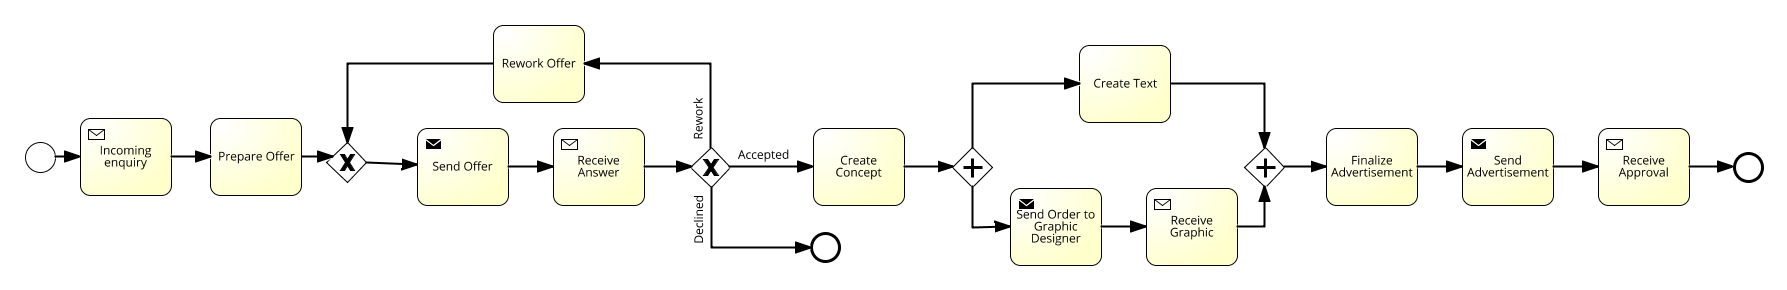
\includegraphics[width=0.9\textwidth]{src/images/private_process_agency.png}
\caption{Private Model Example}
\label{fig:privateModel}
\end{figure}

For example, in the private model shown in Figure \ref{fig:privateModel}, the task \textit{Create Concept} represents a private activity, whereas the task \textit{Send Offer}, involves message exchange with another participant and therefore represents a public activity. A private model is a process model in the classical sense. It's fundamental modeling objects are unchanged since BPMN 1.0. Is a private process modeled and attributed in detail, it also represents an executable process that can be executed by a process engine.

\subsubsection{Public Model}
The public model is also modeled from the perspective of a single participant of a collaborative process. It is a reduced view on the private model of a partner. It can also be described as a projection of the whole collaboration process focusing on one participant. It only includes public activities, involving message exchange with other partners. Private activities which are not relevant for other partners and which don't want be to be shared with the partners are omitted deliberately. Figure \ref{fig:publicModel} shows the corresponding of the already introduced private model. 

\begin{figure}[H]
\centering
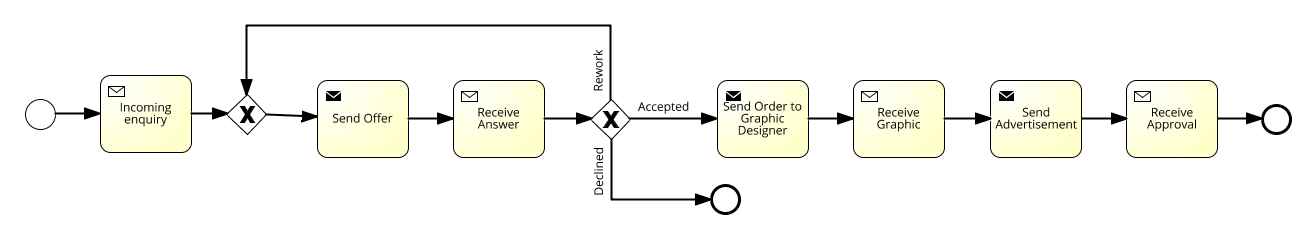
\includegraphics[width=0.9\textwidth]{src/images/public_process_agency.png}
\caption{Public Model Example}
\label{fig:publicModel}
\end{figure}

\subsubsection{Collaboration Model}
The collaboration model is the interconnection between the public models of all participants. The thereby formed model gives a holistic view on the collaborative process and does not focus on one partner. Each partner is represented as a pool and the message exchange between them is shown by a message flow that connects two public activities or just the pools. Figure \ref{fig:collabModel} shows an example collaboration model.

\begin{figure}[H]
\centering
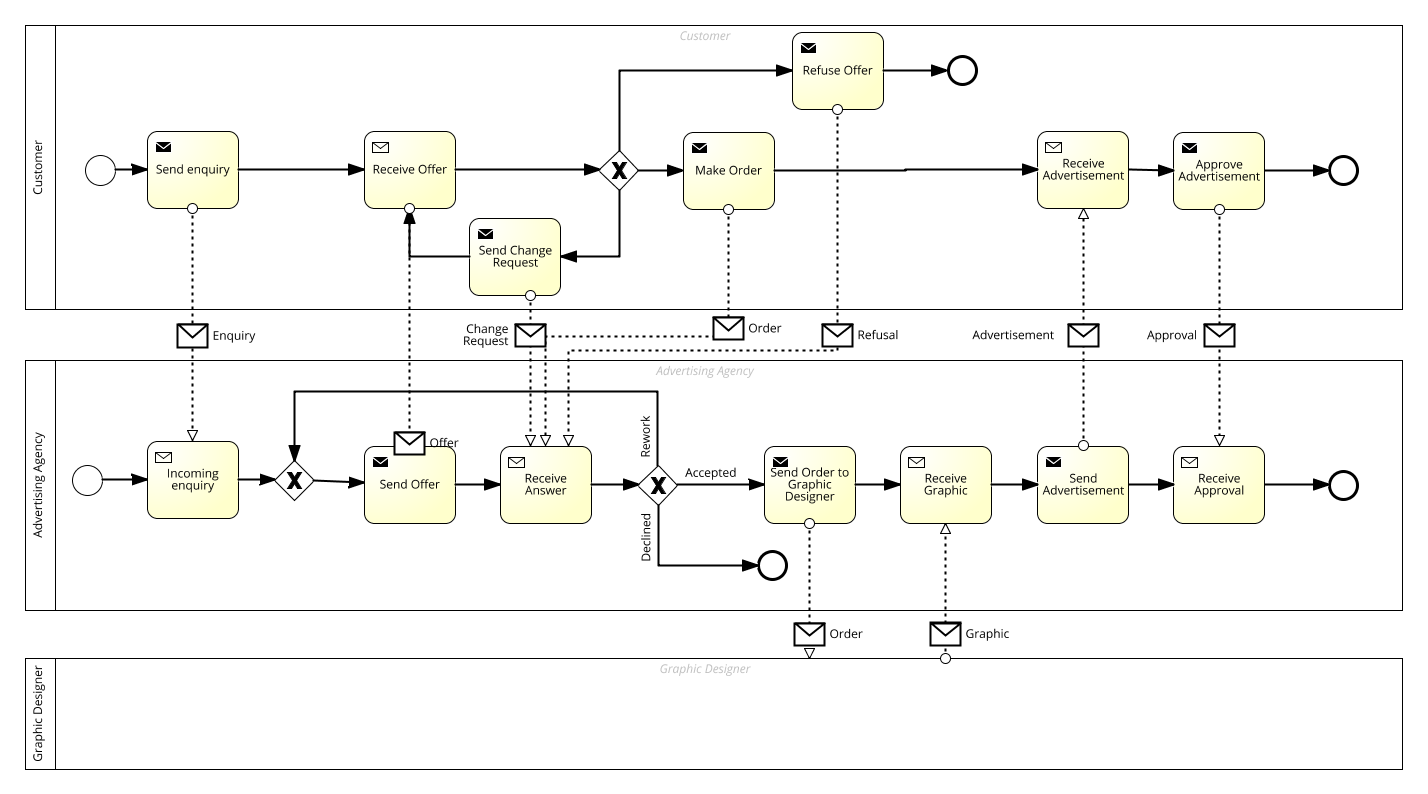
\includegraphics[width=0.9\textwidth]{src/images/collab_advertisement.png}
\caption{Collaboration Model Example}
\label{fig:collabModel}
\end{figure}

Each partner's public process is modeled inside a pool. It is also allowed for a process to not include the public model inside an participant's pool. If a pool contains a process, it is called a "white box". If a pool is empty, it's called a "black box". For Example in figure \ref{fig:collabModel} the pools of the partners \textit{Customer} and \textit{Advertisement Agency} are modeled as "white box" and the pool of the \textit{Graphic Designer} as a "black box" \cite{BPMN20}.

\subsubsection{Choreography Model}
The choreography model is available since BPMN 2.0 and focuses solely on the sequence of message exchanges between the partners. Each message exchange is represented as an interaction with an initiating 
partner, a receiving partner (shaded in grey) and the message exchanged. In contrast to the collaboration model, which also focuses on the message flow, the choreography model additionally displays the exact sequence flow (i.e. conditional message flows or parallel message flows), which is not always evident form the former (i.e. black box pools).

\begin{figure}[H]
\centering
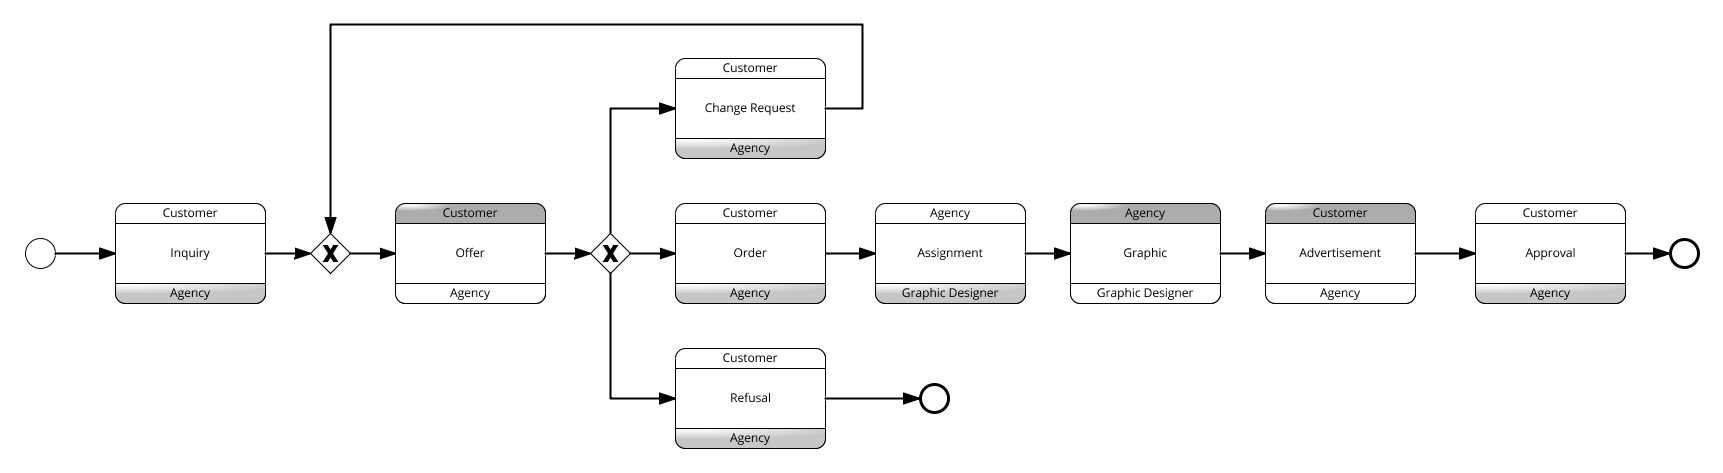
\includegraphics[width=0.9\textwidth]{src/images/choreo_advertisement.png}
\caption{Choreography Model Example}
\label{fig:choreoModel}
\end{figure}